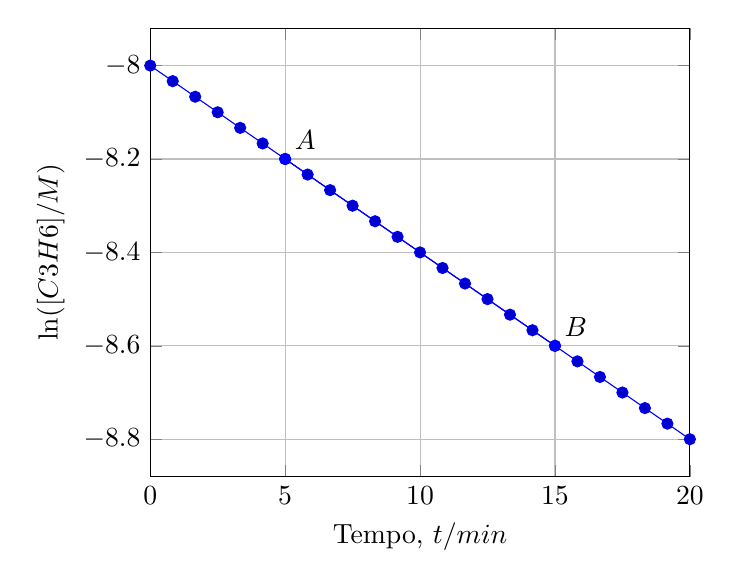
\begin{tikzpicture}
    \begin{axis}
        [
            xlabel = {Tempo, $t/\unit{min}$},
            ylabel = {$\ln([\ce{C3H6}]/\unit{M})$},
            xmin = 0, xmax = 20,
            domain = 0:20,
            grid = major,
        ]

    \addplot+ [blue]
        {
            -8 - 0.04*x
        };

    \addplot [mark=*, color=blue] coordinates
        { 
            (5,-8.2) 
            (15,-8.6)
        };
        
    \node [anchor = south west] at (axis cs:5,-8.2) 
        {$A$};

    \node [anchor = south west] at (axis cs:15,-8.6) 
        {$B$};

    \end{axis}
\end{tikzpicture}